\documentclass[a4paper,11pt]{scrartcl}

\usepackage[utf8]{inputenc}
\usepackage[ngerman]{babel}
\usepackage[T1]{fontenc}
\usepackage{amsmath}
\usepackage{graphicx}
\usepackage{tabularx}
\usepackage[a4paper, left=2cm, right=2cm, top=2.8cm, bottom=2.8cm]{geometry}
\usepackage{tikz}   
\usepackage[scaled]{helvet}
\usepackage{tabto} 
\usepackage{fancyhdr}
\usepackage{multirow}

\renewcommand*{\familydefault}{\sfdefault}

\pagestyle{fancy}

\setkomafont{section}{\huge}
\setkomafont{subsection}{\Large}


\lhead{Maximilian Hoffmann}
\chead{Betrieblicher Auftrag \\ \textbf{Kabeltester}}
\rhead{
\includegraphics[width=3cm]{Bilder/BMK_LOGO.png}}

%%%%%%%%%%%%%%%%%%%%%%%%%%%%%%%%%%%%%%%%%%%%%%%%%%%%%%%%%%%%%%%%%%%%%%%%%%%%%%%%%%%%%%%%%%%%%%%%%%%%%%%%%%%%%%%%%%%%%%%%%%%%%%%%%%%%%%%%%%%%%%%																																			 %
%														Funktionen der Schaltung															%
%																																		     %
%%%%%%%%%%%%%%%%%%%%%%%%%%%%%%%%%%%%%%%%%%%%%%%%%%%%%%%%%%%%%%%%%%%%%%%%%%%%%%%%%%%%%%%%%%%%%%%%%%%%%%%%%%%%%%%%%%%%%%%%%%%%%%%%%%%%%%%%%%%%%%

\begin{document}

%%%%%%%%%%%%%%%%%%%%%%%%%%%%%%%%%%%%%%%%%%%%%%%%%%%%%%%%%%%%%%%%%%%%%%%%%%%%%%%%%%%%%%%%%%%%%%%%%%%%%%%%%%%%%%%%%%%%%%%%%																																						%
%														Versorgung														%
%																														%
%%%%%%%%%%%%%%%%%%%%%%%%%%%%%%%%%%%%%%%%%%%%%%%%%%%%%%%%%%%%%%%%%%%%%%%%%%%%%%%%%%%%%%%%%%%%%%%%%%%%%%%%%%%%%%%%%%%%%%%%%

\section{Schaltplanentwurf}

\begin{center}
In diesem Teilbereich meiner Dokumentation wird auf die Funktion der Schaltung eingegangen. 
\end{center}

\subsection{Versorgung}

\subsubsection{Schutzbeschaltung}

\begin{center}
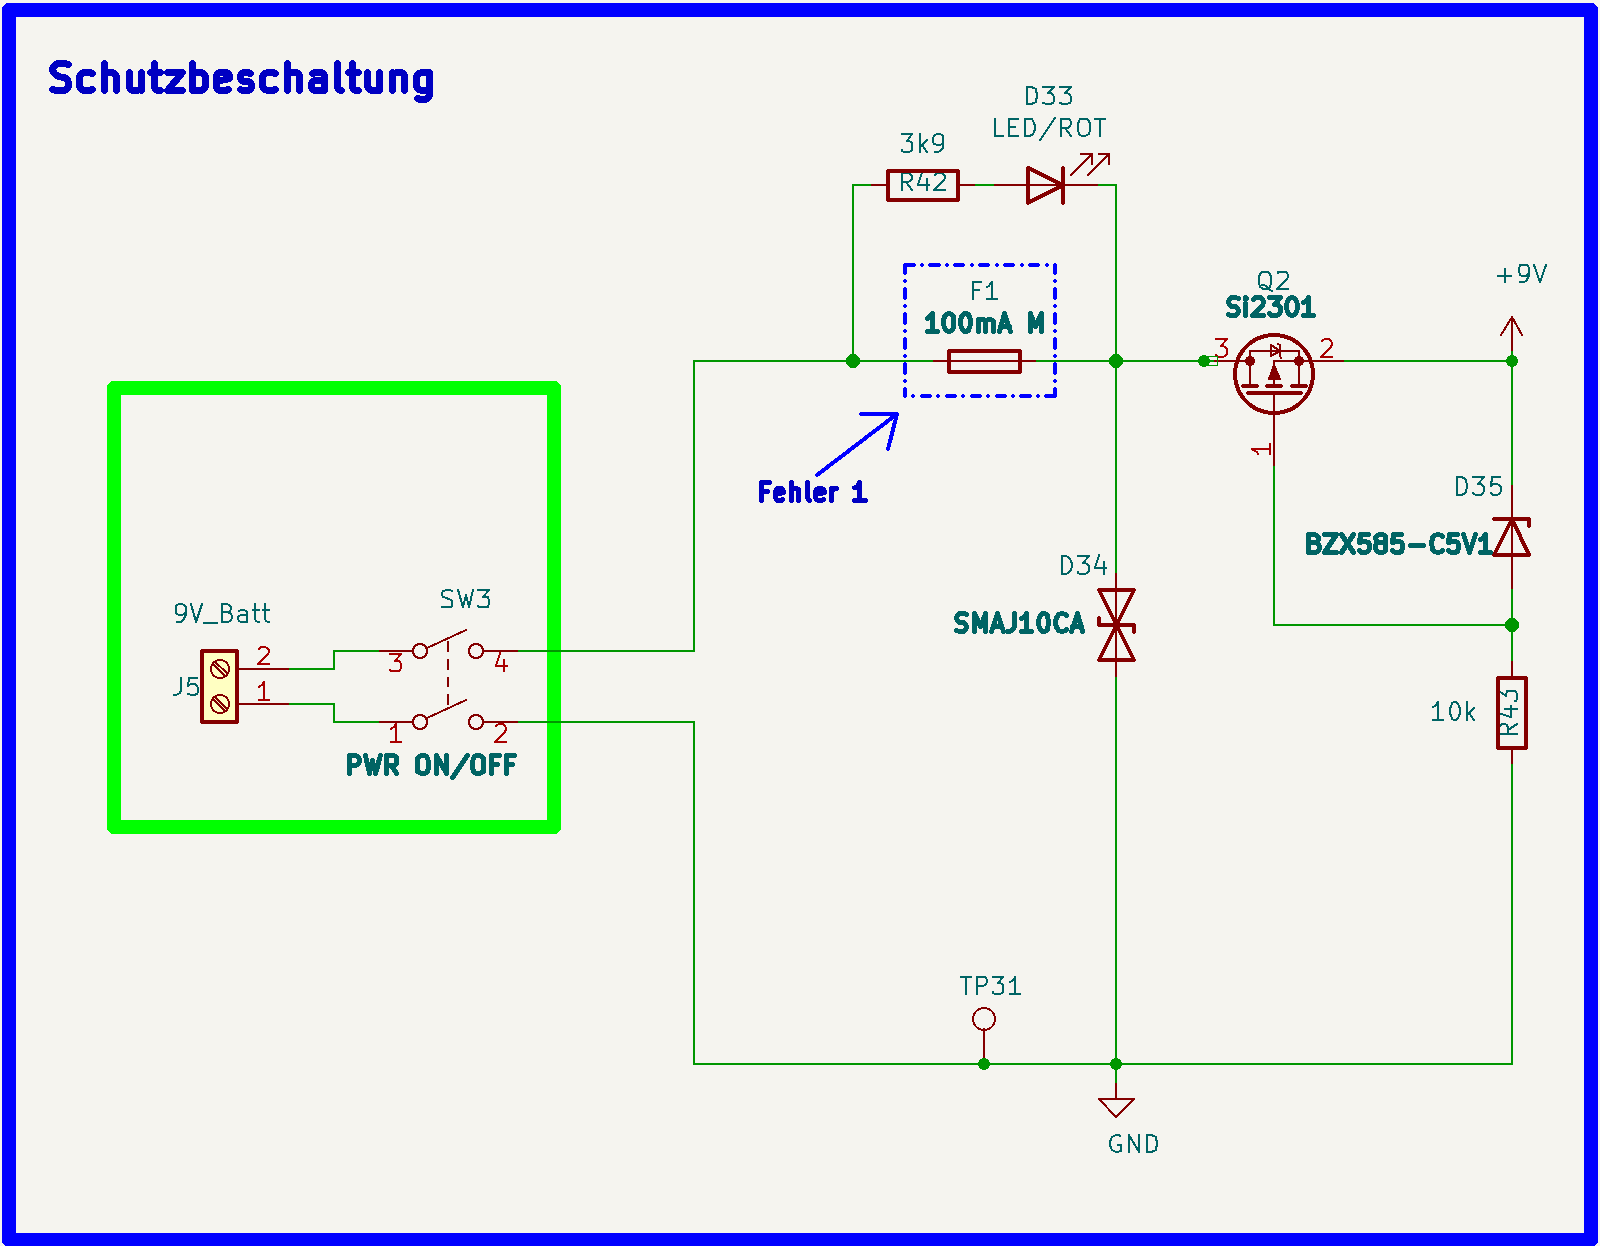
\includegraphics[width=10cm]{Bilder/Schutzbeschaltung.png}
\end{center}

Um die Schaltung zu schützen, wurde auf eine umfangreiche Eingangsschutzbeschaltung gesetzt. Die Versorgungsspannung kann dabei zweipolig durch den Schalter \glqq Power ON/OFF SW3 \grqq{} abgeschaltet werden.
\\
\\
Die mittelträge Sicherung F1 ist für den Überstromschutz verantwortlich. Löst diese aus, so bildet sich ein Strompfad über R42 und D33, welcher den Strom auf ein Maximum von 2mA in der gesamten Schaltung begrenzt. Als Ergebnis wird D33 rot leuchten. Im Normalbetrieb wird der Strompfad R42 - D33 durch den ohmschen Widerstand der Sicherung F1 (12R) überbrückt.
\\
\\
Um den Eingang des DC/DC Wandlers vor Überspannungsspitzen zu schützen wurde auf eine 10V TVS Diode gesetzt. Die Eingangsspannung dieser Schaltung wird dadurch auf ein Spannungsmaximum von 10V begrenzt. 
\\
\\
Da es bei einer Batterieanwendung sehr schnell zu einer ungewollten Verpolung der Anschlüsse kommen kann, ist ein umfangreicher Verpolungsschutz Pflicht. Im Fall einer Verpolung bringt diese Art von Verpolungsschutz zwei große Vorteile mit sich:
\begin{itemize}
	\item{Es muss nicht mit einem festen Spannungsabfall einer in reihe zur Last liegenden Diode gerechnet werden.}
	
	\item{Mit einem hohem Stromfluss, welcher durch eine parallel zur Last liegende Schutzdiode hervorgerufen wird, muss ebenfalls nicht gerechnet werden.}
\end{itemize}
Liegt eine korrekt gepolte Spannung an, so bildet sich ein Strompfad über die Z-Diode D35 und den strombegrenzenden Widerstand R43. Die über die Z-Diode abfallende Spannung von 5,1V liegt somit auch an den Anschlüssen \glqq Source und Gate \grqq{} des P-Channel MOSFET Q2 an. Die Vorgabe für eine leitende Drain - Source Strecke eines P-Channel MOSFET ist ein um ca. 5V positiveres Potential an Source gegenüber Gate. Im korrekt gepolten Fall lässt sich dieser Zustand darauf zurückführen.
\\ 
Im Falle einer Verpolung bildet sich ebenfalls der Strompfad (D35 und R43). Durch die umgekehrte Polung ist nun D35 nicht mehr als Z-Diode, sonder als normale Si-Diode zu betrachten. Somit ist das Potential an Gate um die \glqq Forward Spannung \grqq{} von D35 positiver als Source.  Der P-Channel MOSFET sperrt und ein Stromfluss wird unterbunden.
\\
\\
\subsubsection{DC/DC Wandler}

\begin{center}
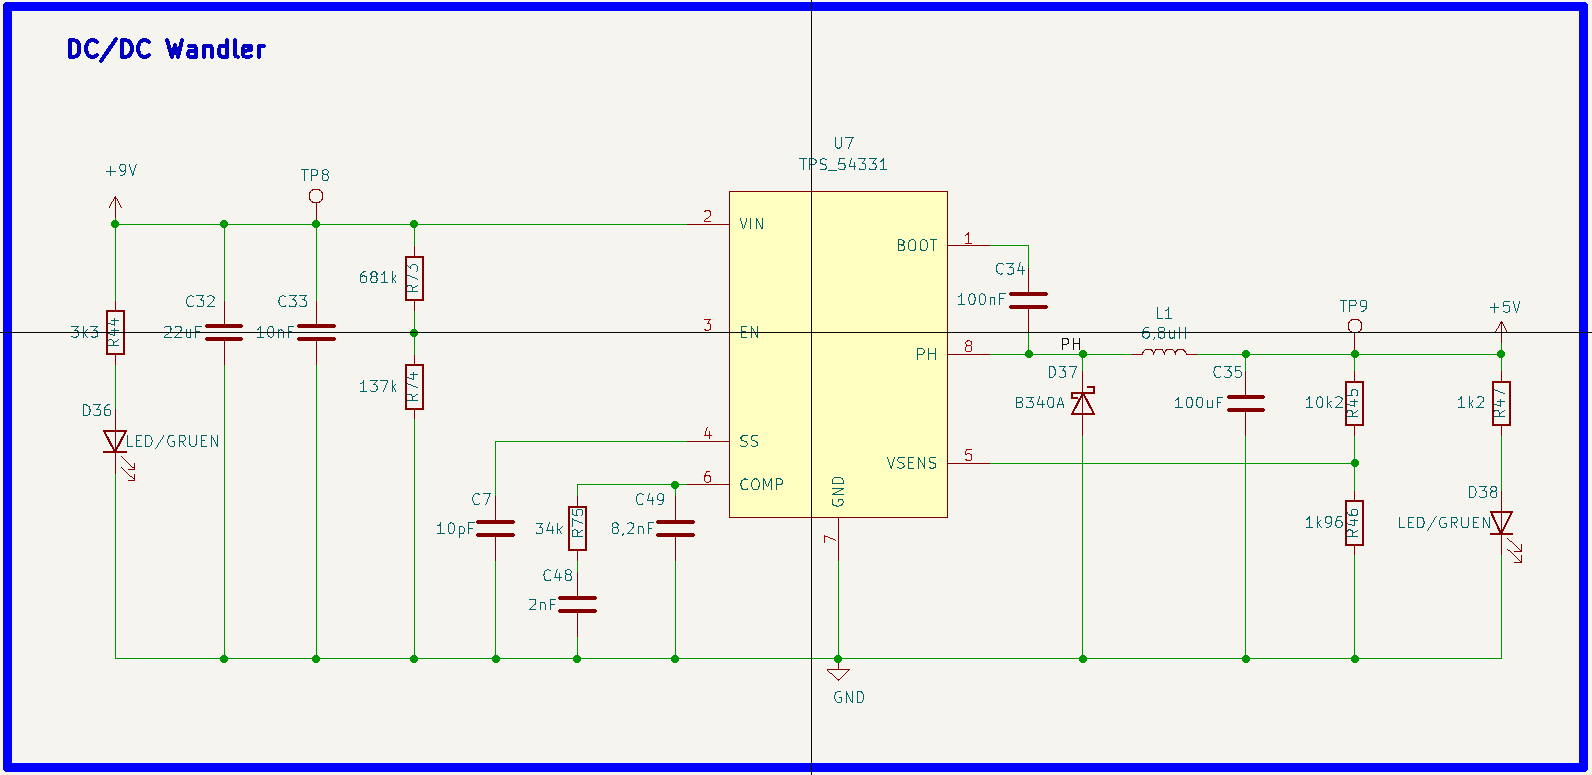
\includegraphics[width=16cm]{Bilder/DCDCWandler.png}
\end{center}

Bei der Auswahl des DC/DC Wandlers wurde auf die Verfügbarkeit bei BMK im Haus geachtet. Die Dimensionierung der externen Bauelemente wurde mit Hilfe des \glqq Texas Instruments Power Designer \grqq{} durchgeführt. Die grünen LED's D36 und D38 sorgen für ein optisches Feedback der Spannungen. Allgemein wurde der Wandler für eine Ausgangsspannung von +5V und einen Ausgangsstrom von ca. 1,5A dimensioniert. Mit den Widerständen R73 und R74 kann der Schaltregler bei Über/-Unterspannung abschalten. Die obere Schwellwertspannung beträgt +10V. Die untere Schwellwertspannung beträgt +8V.

\begin{align}
	R73 &= \dfrac{V_{\Delta}}{3uA} = \dfrac{2V}{3uA} = 666k  \Rightarrow 680k\\
	R74 &= \dfrac{1,25V}{\dfrac{Vs - 1,25V}{R73} + 1uA} = \dfrac{1,25V}{\dfrac{8V - 1,25V}{680k} + 1uA} = 126k \Rightarrow 150k	\\
	V_{OUT}	&= V_{REF} + (\dfrac{R45}{R46} + 1) = 0,8V + (\dfrac{10,2k}{1,96k} + 1) = 4,96V
\end{align}

\newpage

%%%%%%%%%%%%%%%%%%%%%%%%%%%%%%%%%%%%%%%%%%%%%%%%%%%%%%%%%%%%%%%%%%%%%%%%%%%%%%%%%%%%%%%%%%%%%%%%%%%%%%%%%%%%%%%%%%%%%%%%%																																						%
%														NE555 Taktgeber													%
%																														%
%%%%%%%%%%%%%%%%%%%%%%%%%%%%%%%%%%%%%%%%%%%%%%%%%%%%%%%%%%%%%%%%%%%%%%%%%%%%%%%%%%%%%%%%%%%%%%%%%%%%%%%%%%%%%%%%%%%%%%%%%

\subsection{NE555 Taktgeber}

\subsubsection{Takt}

\begin{center}
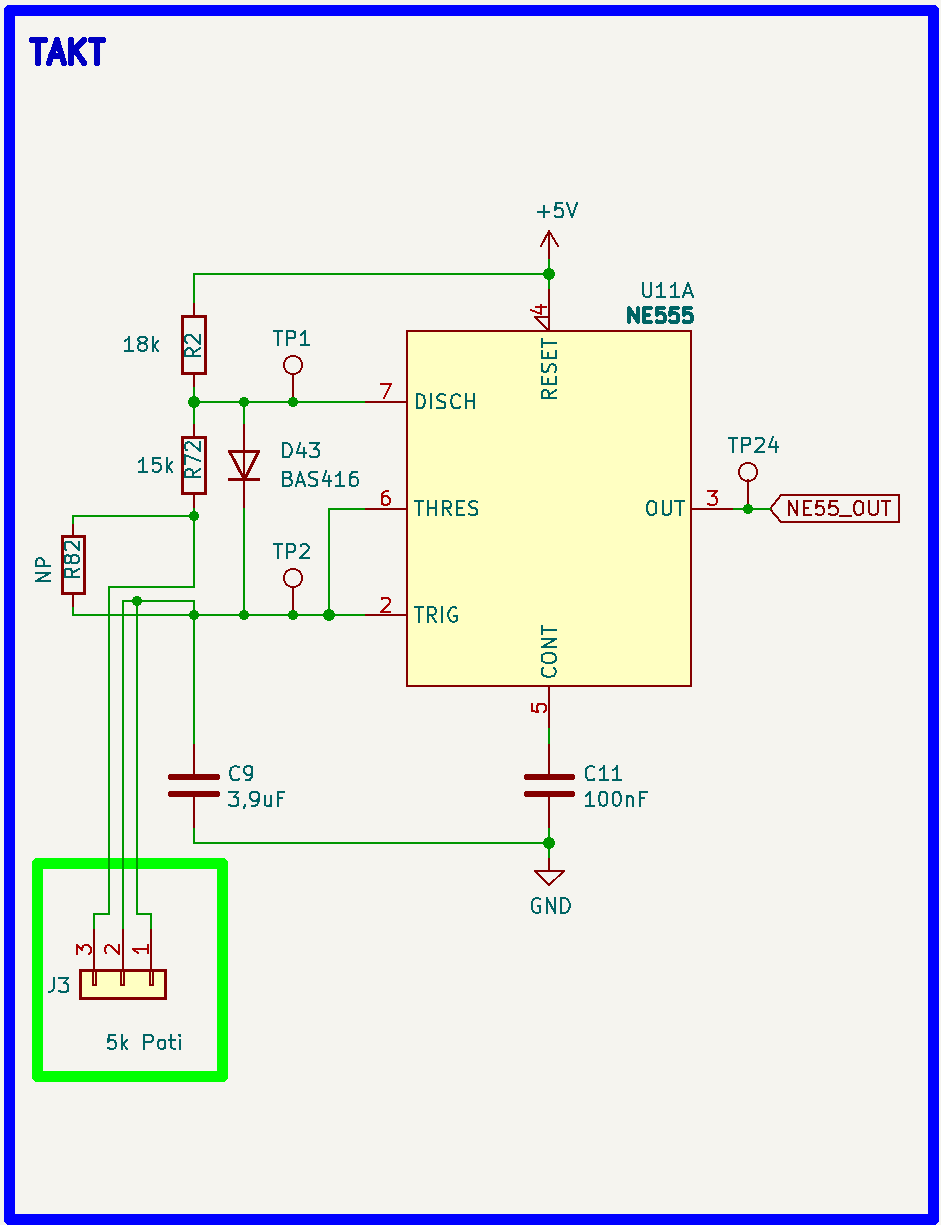
\includegraphics[width=10cm]{Bilder/Takt.png}
\end{center}

Als Taktgeber kommt der \glqq NE555 \grqq{} zum Einsatz. Dieser wird als astabile Kippstufe betrieben. Mit Hilfe der Diode D43 gleichen sich Impulszeit und Pausenzeit an. Über das Poti (Connector) J3 soll die Ausgangsfrequenz auf ca. 10Hz eingestellt werden können. 

\begin{align}
	f_{OUT} &= \dfrac{1}{0,69*R2*C9 + 0,69*(R72+R_{J3})* C9} = \dfrac{1}{0,69*18k*3,9uF*2} = 10,3Hz
\end{align} 




\end{document}